\documentclass[12pt,a4paper]{article}
\usepackage{pgf}
% \usepackage[condensed,math]{kurier}
% \usepackage[T1]{fontenc}
\usepackage{svg}
\usepackage{tikz}
\usepackage{stanli}
\usepackage{afterpage}
\usepackage{multirow}
\usepackage{subfig}
\usepackage{pgfpages}
\usepackage{svg}
\usepackage{rotating}

%\usepackage{times}


\pgfpagesdeclarelayout{boxed}
{
	\edef\pgfpageoptionborder{0pt}
}
{
	\pgfpagesphysicalpageoptions
	{%
		logical pages=1,%
	}
	\pgfpageslogicalpageoptions{1}
	{
		border code=\pgfsetlinewidth{2pt}\pgfstroke,%
		border shrink=\pgfpageoptionborder,%
		resized width=.9\pgfphysicalwidth,%
		resized height=.9\pgfphysicalheight,%
		center=\pgfpoint{.5\pgfphysicalwidth}{.5\pgfphysicalheight}%
	}%
}

\pgfpagesuselayout{boxed}


% Language setting
% Replace `english' with e.g. `spanish' to change the document language
\usepackage[portuguese]{babel}

% Set page size and margins
% Replace `letterpaper' with `a4paper' for UK/EU standard size
\usepackage[a4paper,top=2cm,bottom=1.5cm,left=1.5cm,right=1.5cm,marginparwidth=1.75cm]{geometry}

% Useful packages
\usepackage{amsmath}
\usepackage{graphicx}
\usepackage[colorlinks=true, allcolors=black]{hyperref}

\title{}
\author{}
\date{}

\begin{document}
	
	\newcommand{\subf}[2]{%
		{\small\begin{tabular}[t]{@{}c@{}}
				#1\\#2
		\end{tabular}}%
	}
	
	\begin{titlepage}
		\begin{center}
			\vspace*{3cm}
   
			\Huge
			\textbf{Projeto de Laboratórios de Informática III}
			\vspace{0.3cm}
			\Huge
   
			Fase 1
			\vspace{0.8cm}
   
			\large
			\vspace{1.5cm}
			\LARGE
			\vspace{1.5cm}
			\textbf{}
            \includegraphics[width=0.4\textwidth]{image.png}
			\vfill
			\vspace{1.0cm}
			\Large
			
		\end{center}
		\Large
		\begin{tabbing}
			\hspace*{1em}\= \hspace*{8em} \= \kill % set the tabbings
            \> Grupo: \textbf{44} \\
			\> Desenvolvido por: \textbf{Afonso Dionísio Santos, A104276} \\
            \>\>\textbf{Mário André Leite Rodrigues, A100109} \\
            \>\>\textbf{Pedro Figueiredo Pereira, A104082} \\
			
		\end{tabbing}
		
	\end{titlepage}
	
	\tableofcontents
	\newpage
    \section{Introdução}
    \hspace{0,6cm}Na unidade curricular de Laboratórios de Informática III, foi proposto realizar um projeto em C, para consolidar conhecimentos essenciais da linguagem prevista, assim como, desenvolvimento de aptidões no âmbito de engenharia de \textit{Software}, tais como modularidade e encapsulamento, estruturas dinâmicas de dados, validação funcional e medições de desempenho computacional. Prevê-se também a habilitação dos intervenientes relativamente à utilização de ferramentas essenciais ao desenvolvimento de projetos neste formato, nomeadamente, ferramentas de compilação, linkagem, depuração de erros, avaliação de desempenho, consumo de recursos e gestão de repositórios colaborativos. \\
        
    Na primeira fase do projeto, foi planeada e executada a idealização da estrutura a utilizar na aplicação do grupo, estruturação inicial do projeto, leitura e filtragem de dados de ficheiros para a memória e consequente resposta a seis das \textit{queries} sugeridas pela equipa docente.\\
        
    O relatório irá abordar decisões e estratégias pelas quais o grupo optou para concretização dos pontos referidos anteriormente com sucesso.
         
    \section{Desenvolvimento}
    \hspace{0,6cm}Dado todos os desafios referidos previamente, entre grupo, decidiu-se a produção de um delineamento prévio de estruturação do projeto que nos permitisse solucionar o problema apresentado da forma mais clara e eficiente possível. Segue nesta secção a orientação e execução do nosso plano.  

    \subsection{Arquitetura do projeto}

    \hspace{0,6cm}Esta sub-secção é dedicada à exposição das estruturas de dados utilizadas, diagrama de dependências dos módulos presentes no nosso projeto e diagrama expositivo da dinâmica geral da aplicação.
    
    \subsubsection{Estrutura de Dados}

    \hspace{0,6cm}Devido à natureza do projeto em utilizar alocação de memória para desenvolvimento da aplicação, foi necessário decidir as estruturas a utilizar para representar da melhor forma possível a informação que chega dos CSV's e é posteriormente filtrada e guardada na memória de forma integra e organizada. \\

    Nesta fase inicial do projeto, a nossa implementação passou por respeitar o tipo associado aos dados atribuídos nos CSV's e desta forma, manter as definições dos nossos parâmetros de acordo com essa normal inicial, como tal, maioritariamente, mantivemos a utilização de strings (char*) como definição predileta para representação e especificação dos dados.\\

    Objetivamente, o primeiro ficheiro CSV a ser desconstruído para a memória foi o "/flghts.csv", onde, optámos inicialmente por alocar, com definição char* todos os dados relativo a este modelo. Posteriormente, com o avanço do desenvolvimento e contextualização conclui-se a incoerência de alocar dados não utilizados. Como tal, foram removidas todas as ocorrências de tentativas de guardar na memória  que não são utilizados no decorrer da aplicação. Numa fase final, observou-se a necessidade e melhoria de alocação noutras definições como inteiros (int) ou doubles (double) para utilização eficiente e simplificada nas repostas às queries. Como panorama final, apresentam-se os campos flight\_id, airline, plane\_model, origin, destination, schedule\_departure\_date, schedule\_arrival\_date, real\_departure\_date e real\_arrival\_date como strings do tipo (char*) e o campo total\_seats como inteiro do tipo int.\\

    O segundo ficheiro a ser trabalhado foi o de "/passengers.csv", tal como na implementação anterior optou-se por alocar os valores de flight\_id e user\_id como strings do tipo (char*).\\

    Segue-se a definição dos parâmetros do ficheiro de "/reservations.csv", onde, elaborámos as mesmas decisões e execuções do primeiro, finalmente, escolhemos os campos reservation\_id, user\_id, hotel\_id, hotel\_name, begin\_date, end\_date e includes\_breakfast como strings do tipo char* e os campos hotel\_stars, city\_tax, price\_per\_night e rating como inteiros do tipo int.\\

    Por último, procedeu-se à desconstrução do ficheiro de "users.csv" através da aplicação da estratégia de uniformização de e manutenção dos estados iniciais e, como tal, definiram-se os campos user\_id, name, birth\_date, sex, passport, country\_code, account\_creation e account\_status como strings do tipo char*.\\
    
    \subsubsection{Diagrama Geral}
    \hspace{0,6cm}Após leitura atenta do enunciado e contextualização das funcionalidades e recursos necessários, decidiu-se dividir a aplicação em cinco contextos principais: modelos, controladores, serviços, stats e utils.\\

    Nos modelos podemos encontrar aquela que é a definição de cada um dos ficheiros (flights, passengers, reservations e users) quando desconstruídos para o nosso código, ou seja, as estruturas, os setters, getters e funções de libertação de memória que permitem respeitar o encapsulamento e trabalhar os dados.\\

    Nos controladores estão todas as funções que permitem gerir e controlar os dados associados à nossa aplicação, organização de dados em estruturas personalizadas (Exemplo: HashTables/Listas/Arrays), setters, getters e funções de libertação de memória que permitem respeitar o encapsulamento e facilitar o workflow de desenvolvimento da plataforma.\\

    Nos serviços estão explícitos os diferentes serviços categorizados por partes funcionais da aplicação, todos as funções ou necessidades são apresentadas aqui, como por exemplo, o parser, as funções de alimentação de estruturas, as respostas às queries e a escrita para ficheiros.\\

    Nas estatísticas apresentamos todas as funcionalidades que permitem gerir os dados relativos a cada tipo de ficheiro e complementam a resposta às queries.\\

    Nas utilidades estão implementadas todas as funções e requisitos necessários para apoio a outros contextos do projeto.\\

    Segue em baixo um diagrama que representa a arquitetura atual da nossa aplicação com o intuito de simplificar o entendimento e fluidez nos diferentes detalhes do projeto.\\

    \begin{center}
    \centering
    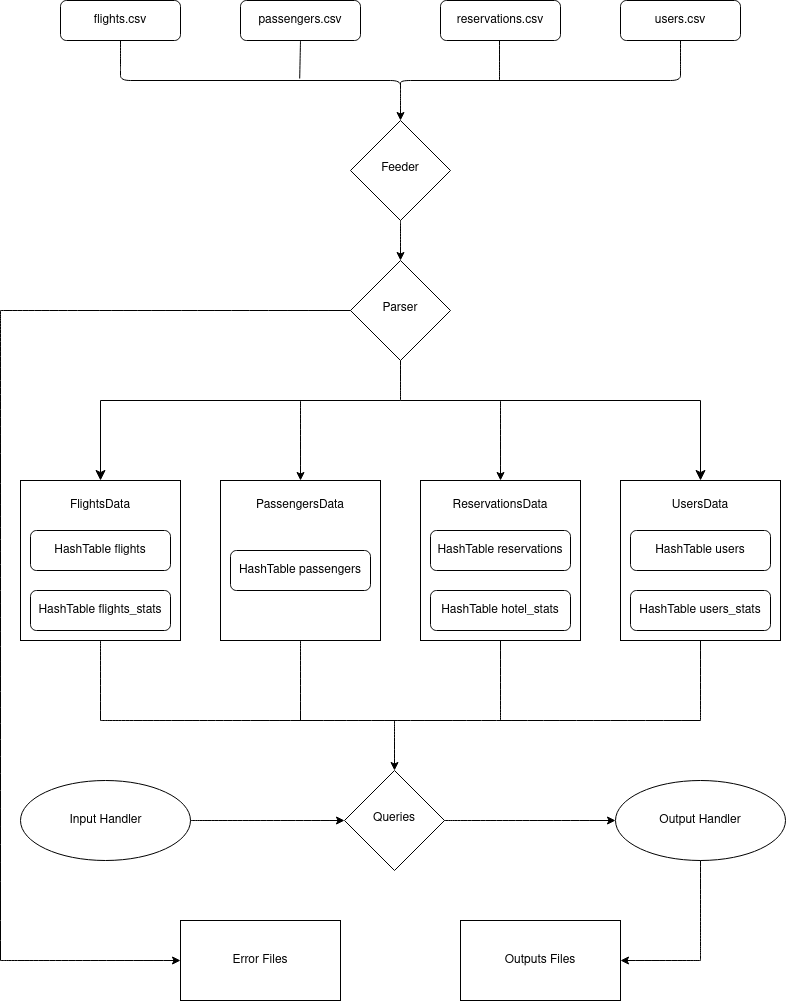
\includegraphics[scale=0.6]{arquitetura_geral.png}
    \end{center}

    \begin{center}
    Figura 1: Diagrama da estrutura da aplicação.
    \end{center}
    
    \subsection{Estratégias seguidas nas queries}
    \subsubsection{Query 1}
    \hspace{0,6cm}Na Query 1, inicia-se o processo de resposta com receção do parâmetro correspondente à query, sendo ele, opcionalmente, o ID de um utilizador, reserva ou voo. Com o objetivo de listar o resumo de uma destas entidades, inicia-se a resolução verificando o tipo de ID que foi atríbuido na chamada da query, permitindo a procura concreta de dados necessários e adaptação à necessidade da query.\\
    
    Transversalmente, existe uma separação em dois conteúdos nesta query, os dados de obtenção direta e os dados calculados estatisticamente, esta divisão surge da necessidade de otimizar a resolução do problema de forma a agrupar pesquisas de múltiplos dados e otimizar a sua obtenção.\\

    Os dados de obtenção direta são conseguidos por pesquisa da estrutura informativa nos diferentes conjuntos de dados, tais como, ReservationsData, FlightsData e UsersData, através de HashTables pertencentes à estrutura de cada modelo, entre elas, reservations, flights e users, e consequente acesso aos dados que contêm toda a informação correspondente, nomeadamente, ReservationInfo, FlightInfo e UserInfo. Para tal, utiliza-se uma função que permite o acesso a cada estrutura informativa a que o ID correspondente e procede-se à extração encapsulada dos elementos necessários para reposta.\\

    Relativamente aos dados calculados estatisticamente, com o intuito de melhorar a performance do grupo e organização estrutural, procurámos alimentar alguns elementos estatísticos no momento de alocação orientada na memória. Para facilitar os dados requisitados foi adicionado a cada conjunto de dados referidos anteriormente um detalhe estatístico. Como tal, número de passageiros num voo, número de reservas e voos de um utilizador são extraídos em tempo constante na execução da query. Em contrapartida, verifica-se uma maior utilização de memória e aumento do tempo de arranque da aplicação.\\

    Em suma, a Query 1 pretende, de forma eficaz, listar informações importantes e práticas de qualquer extrato de informação atribuído inicialmente à aplicação. A implementação apresentada pretende corresponder a estas expectativas e solucionar o problema no melhor rácio entre velocidade de resposta e uso de memória possível.
    
    \subsubsection{Query 2}
    \hspace{0,6cm}Na Query 2, inicialmente, é verificado o tipo de pesquisa a ser executada, podendo abranger voos, reservas ou ambas as opções. Essa diferenciação permite uma adaptação flexível da busca às necessidades específicas do usuário.\\
    
    Visando otimizar o desempenho da busca e garantir uma eficiência constante, ao inserir novos usuários, procedemos à inclusão dos identificadores (IDs) dos voos em um GArray denominado "user flights". De maneira análoga, os IDs das reservas são armazenados em um GArray denominado "user reservations". Essa abordagem estratégica não apenas facilita a recuperação rápida de informações, mas também contribui para a agilidade no processamento da query.\\
    
    Durante a execução da query, a operação se concentra em aceder à Hashtable para localizar o user específico, sendo desnecessário uma procura extensiva dos dados. A iteração subsequente nos arrays "user flights" e "user reservations" proporciona uma coleta eficiente das informações pertinentes ao tipo de procura.\\
    
    Ao finalizar a execução, os resultados são submetidos a uma ordenação criteriosa por data, e o conjunto final é então impresso no ficheiro correspondente à query. Essa etapa final, com a ordenação, adiciona uma camada de organização aos resultados, facilitando a interpretação e análise por parte do usuário ou de sistemas externos que possam consumir esses dados.\\
    
    Em resumo, a abordagem adotada na Query 2 não apenas assegura a eficácia na recuperação de informações específicas para cada user, mas também promove a otimização do processo, visando proporcionar uma experiência de busca eficiente e resultados organizados.\\

    \subsubsection{Query 3}
    \hspace{0,6cm}Na Query 3, o processo tem início ao receber o ID de um Hotel como entrada, visando calcular a média dos ratings associados a este estabelecimento.\\

    O desafio central reside na determinação do número de visitantes que frequentaram o hotel em questão, assim como o cálculo da soma dos ratings correspondentes atribuídos por diversos utilizadores.\\

    Com o objetivo de otimizar o desempenho, implementamos uma abordagem que implica a criação de uma nova estrutura de dados denominada "hotel\_stats", baseada numa Hashtable. Esta estrutura é construída mediante a inserção de dados, efetuando, simultaneamente, o cálculo do número de clientes que visitaram o hotel e a soma total dos ratings obtidos. Esses ratings representam o somatório das avaliações dos utilizadores específicos para aquele hotel em particular.
       
    \subsubsection{Query 4}
    \hspace{0,6cm}Na Query 4, a funcionalidade é voltada para a obtenção de estatísticas específicas de um hotel, identificado pelo parâmetro "id". Inicialmente, são adquiridas as estatísticas do hotel por meio da função "get hotel stats by hotel id", seguida pela obtenção das reservas associadas a esse hotel através da função "get hotel reservations".
        
    A seguir, são alocados dinamicamente recursos para a estrutura QUERY4 RESULT, que armazenará os resultados da query. Os arrays dentro dessa estrutura, como "reservation id", "begin date", "end date", "user id", rating, e "total price", são dimensionados de acordo com o número de reservas obtidas. Um loop subsequente percorre essas reservas, filtrando aquelas que possuem IDs iniciados por "Book". Para cada reserva válida, são extraídas informações relevantes, como datas de início e término, ID do usuário, avaliação, preço por noite e preço total.\\
    
    As informações processadas são armazenadas na estrutura QUERY4 RESULT. Após o loop, a estrutura é submetida a uma ordenação por data e valor, utilizando a função "sort by date and value". Os resultados finais são então registrados no arquivo de saída por meio da função "write query4".\\
    
    Por fim, a liberação cuidadosa de memória é realizada para evitar vazamentos. Os arrays internos da estrutura QUERY4 RESULT e a própria estrutura são desalocados utilizando a função free.\\
    
    Em resumo, a Query 4 é responsável por fornecer estatísticas detalhadas de reservas para um hotel específico, incluindo informações como datas, IDs de reserva, IDs de usuário, avaliações e preços totais. O código é estruturado de maneira a garantir uma manipulação eficiente da memória e uma produção precisa dos resultados.

    \subsubsection{Query 8}
    \hspace{0,6cm}A Query 8 tem como objetivo calcular a receita gerada por um hotel em um intervalo de datas específico, identificado pelo parâmetro "id" do hotel e pelas datas de início e término, representadas pelos parâmetros "begin\_date" e "end\_date", respectivamente.\\

    No início da função, são obtidas as estatísticas do hotel por meio da função get\_hotel\_stats\_by\_hotel\_id e, em seguida, são recuperadas as reservas associadas a esse hotel utilizando a função get\_hotel\_reservations. Caso não existam reservas, a função retorna imediatamente.\\

    A variável revenue é inicializada como 0 e é utilizada para acumular a receita durante a iteração sobre as reservas do hotel no período especificado. O loop percorre todas as reservas e verifica se o ID da reserva inicia com "Book" para garantir que seja uma reserva válida.\\

    Dentro do loop, são obtidas as informações relevantes de cada reserva, como as datas de início e término, o preço por noite e o ID da reserva. O código então compara as datas da reserva com o intervalo especificado na query para determinar se a reserva contribui para a receita durante esse período.\\

    As condições dentro do loop consideram diferentes cenários, como reservas que cobrem totalmente o período especificado, reservas que incluem apenas uma noite do intervalo e reservas que se sobrepõem parcialmente ao período. Com base nessas condições, a receita é calculada e acumulada na variável revenue.\\

    Ao final do loop, o valor total da receita acumulada é passado para a função write\_query8, que é responsável por registrar essa receita no arquivo de saída, atendendo ao formato de saída necessário.\\

    Em resumo, a Query 8 realiza uma análise detalhada das reservas de um hotel em um intervalo de datas específico, calculando a receita gerada durante esse período e registrando esse valor no arquivo de saída. O código é estruturado para lidar com diversas situações possíveis, garantindo uma resposta precisa à consulta realizada.

    \subsubsection{Query 9}
    \hspace{0.6cm}Na formulação da Query 9, delineamos o objetivo de listar todos os usuários que possuem um prefixo especificado indicado no input por ordem alfabética.\\
     
    Neste contexto, adotamos uma abordagem distinta em relação à implementação de Hashtable anteriormente mencionadas. Optamos, neste caso, por uma estrutura alternativa, designadamente o GArray, para armazenar informações cruciais sobre o utilizador durante o processo de inserção. Esta escolha justifica-se pela necessidade de preservar dados sensíveis, como user\_id e user\_name, visto que, ao abordarmos a eficiência de iteração nas estruturas de dados, constatamos que percorrer todos os elementos de um GArray demonstra ser mais eficiente do que a abordagem baseada numa Hashtable. Tal eficiência resulta do facto de a Hashtable implicar um mecanismo de indexação que, embora potencialmente robusto, provoca uma diminuição no desempenho.\\

    Posteriormente, procedemos à ordenação do GArray, baseando-nos na ordem alfabética dos nomes dos utilizadores. Em situações em que ocorre a duplicidade de nomes, implementamos uma ordenação adicional, utilizando o user\_id como critério de desempate. \\
     
    Com o array agora ordenado, retomamos a iteração sobre o mesmo, procurando os nomes que correspondem ao prefixo fornecido pelo input.
        
    \subsection{Possiveis otimizações}
    \hspace{0,6cm}No que concerne às possíveis melhorias no projeto, identificamos áreas específicas que poderiam ser refinadas para aprimorar a eficiência e a qualidade do código desenvolvido. Uma destas áreas inclui a otimização da implementação das queries, sobretudo a Query 9, que se revelou menos eficiente em comparação com as restantes. Esta otimização envolveria a revisão e reestruturação da lógica subjacente a esta query, visando uma abordagem mais eficaz na manipulação e tratamento de dados.\\

    Além disso, consideramos viável aprofundar a implementação do encapsulamento de forma a garantir uma maior segurança e coesão no código. Esta otimização poderia ser alcançada por meio de uma análise minuciosa das estruturas de dados e das interações entre os diversos módulos do projeto, visando um melhor encapsulamento e abstração dos dados.\\

    Outra área de potencial melhoria reside na gestão de memória. Embora tenhamos minimizado os vazamentos de memória ao longo do desenvolvimento, reconhecemos a importância de uma revisão mais detalhada do código para identificar e corrigir quaisquer potenciais pontos de ineficiência na alocação e libertação de recursos de memória.
        
    \subsection{Dificuldades sentidas}
      
    \hspace{0,6cm}Durante a realização desta fase do projeto, deparamo-nos com desafios consideráveis que demandaram uma abordagem minuciosa e aprofundada. Um dos principais obstáculos encontrados foi a necessidade de implementar o encapsulamento de forma coerente e eficaz. Este conceito, essencial para a organização e segurança do código, revelou-se complexo para o grupo, dada a relativa falta de familiaridade inicial com o seu funcionamento. A sua implementação, embora benéfica em termos de segurança e estruturação do código, também acarreta uma possível diminuição na velocidade de execução, o que exigiu um equilíbrio delicado entre esses dois pontos.\\

    Outra dificuldade significativa surgiu na otimização da eficiência das queries implementadas. Fomos desafiados a aprimorar as nossas habilidades na elaboração de queries mais eficientes, especialmente no contexto do módulo estatístico. A busca por métodos mais ágeis e otimizados demandou tempo e esforço adicional, mas foi crucial para garantir uma melhor performance do sistema.\\

    Um desafio constante ao longo do desenvolvimento foi a gestão eficaz da memória. A alocação inadequada e a não libertação correta de recursos de memória resultaram em potenciais instabilidades no software. Para mitigar esse problema, foi necessário realizar uma análise minuciosa do código, identificando pontos de melhoria e implementando correções adequadas.\\

    Em suma, as dificuldades encontradas nesta fase inicial do projeto proporcionaram valiosas aprendizagens em termos de estruturação de código, otimização de queries e gestão de recursos. Estes desafios serviram como oportunidades de aprimoramento das nossas competências técnicas, destacando a importância da atenção aos detalhes e da busca contínua por melhorias para alcançar um software mais eficiente e robusto.
    
        
    \section{Conclusão}

    \hspace{0,6cm}Em conclusão, após o desenvolvimento desta primeira fase do projeto de Laboratórios de Informática III, é evidente o avanço significativo no entendimento e aplicação de conceitos fundamentais da engenharia de software e da linguagem de programação C. A abordagem modular adotada permitiu não apenas uma melhor compreensão da estruturação do projeto, mas também destacou a importância do encapsulamento e da eficiência na manipulação de dados.\\

    Enfrentamos desafios consideráveis ao implementar o encapsulamento e garantir a gestão adequada da memória, mas estas dificuldades foram valiosas para o aprimoramento das nossas habilidades e compreensão dos mecanismos de otimização de código. A busca por melhorias nas queries, especialmente na Query 9, demonstrou a necessidade contínua de aperfeiçoar a eficiência do código para lidar com volumes maiores de dados.\\

    É relevante destacar a importância de uma constante revisão e otimização do código, visando não apenas a funcionalidade, mas também a performance e a capacidade de escalar o projeto para demandas futuras. Esta fase inicial foi essencial para sedimentar bases sólidas, e estamos confiantes de que os desafios enfrentados nos proporcionaram um aprendizado valioso para as etapas subsequentes do projeto.
	
	\newpage
        
\end{document} 
